\documentclass[a4paper,10pt]{article}
\usepackage[utf8]{inputenc}
\usepackage{todonotes}
\usepackage{fullpage}
\usepackage{graphicx}
\usepackage{float}
\usepackage{multirow}
\usepackage{wrapfig,booktabs}
\usepackage{tikz}
\usepackage{circuitikz}
\usepackage{cite}
\usepackage{tikz-timing}
\usepackage{url}
\usepackage{hyperref}
\usepackage{subcaption}
\hypersetup{
    colorlinks,
    citecolor=black,
    filecolor=black,
    linkcolor=black,
    urlcolor=black
}

\usepackage{pgf}
\usetikzlibrary{arrows,automata}
\usetikzlibrary{patterns}
\usetikzlibrary{shapes.geometric}
\usetikzlibrary{fit}
\usetikzlibrary{calc}
\usetikzlibrary{intersections}
\usetikzlibrary{backgrounds}
\usetikzlibrary{arrows, decorations.markings}
\usetikzlibrary{decorations.pathreplacing}
\usetikzlibrary{automata} %state machine stuff
\usetikzlibrary{positioning} %midway
\tikzstyle{vecArrow} = [thick, decoration={markings,mark=at position
   1 with {\arrow[semithick]{open triangle 60}}},
   double distance=1.4pt, shorten >= 5.5pt,
   preaction = {decorate},
   postaction = {draw,line width=1.4pt, white,shorten >= 4.5pt}]
\tikzstyle{module} = [rectangle, minimum width = 2 cm,minimum height = 2 cm, draw]

%opening
\title{Brick sorter}
\author{Nikolaj Iversen, Matthias Harald Hessels}


%Todo notes
\usepackage{nameref}
\makeatletter
\newcommand*{\currentname}{\@currentlabelname}
\makeatother

\newcommand{\nikolaj}[1]{\todo[inline,color=red!20,author=Nikolaj]{\currentname: ~ #1}}
\newcommand{\matthias}[1]{\todo[inline,color=blue!20,author=Matthias]{\currentname: ~ #1}}

\newcommand{\figscale}{0.8}

\usepackage{diagbox}
\usepackage{amsmath}
\usepackage{todonotes}
\usepackage{epstopdf}
\usepackage{graphicx}
\usepackage[T1]{fontenc}


\let\ig\includegraphics
\renewcommand{\includegraphics}[2][]{ \IfFileExists{#2}{ \ig[#1]{#2} }{ 
                \IfFileExists{#2.eps}{ \ig[#1]{#2} }{ 
		\IfFileExists{#2.png}{ \ig[#1]{#2} }{ 
		\IfFileExists{#2.jpg}{ \ig[#1]{#2} }{ 
		\IfFileExists{#2.jpeg}{ \ig[#1]{#2} }{ 
		\IfFileExists{#2.gif}{ \ig[#1]{#2} }{ 
		\IfFileExists{#2.ppm}{ \ig[#1]{#2} }{ 
		\IfFileExists{#2.pdf}{ \ig[#1]{#2} }{ 
		\missingfigure{  \protect\detokenize{#2} was not found.} 
}}}}}}}}
}

\newcommand{\missingequation}[1]{\todo[inline, color = yellow]{Missing equation: #1}}


%%
%% End of file `mypackage.sty'.
\tikzset{robot/.style={ 
    minimum width = 1.5cm, minimum height =2cm,
%     fill=blue!10,
    draw, 
    % wheels
    % wheels
    append after command={
      [shorten >=0.5cm, shorten <=0.5cm]
      (\tikzlastnode.north west)edge[very thick, color=black!70](\tikzlastnode.south west)
    },
    append after command={
      [shorten >=0.5cm, shorten <=0.5cm]
      (\tikzlastnode.north east)edge[very thick, color=black!70](\tikzlastnode.south east)
    },
    append after command={
      (\tikzlastnode.north west) ++(0.4,-0.25) circle(0.25cm)
    },
    append after command={
      (\tikzlastnode.north east) ++(-0.4,-0.25) circle(0.25cm)
    },
    append after command={
      (\tikzlastnode.north east) ++(0.25,0.25) circle(0.25cm)
    }
  }
}
 %tikz style for robot
\begin{document}

\begin{titlepage}
	\centering
	{\scshape\LARGE University of Southern Denmark \par}
	\vspace{1cm}
	{\scshape\Large Introduction to Artificial intelligence (RMAI1) \par}
	\vspace{1.5cm}
	{\huge\bfseries Sokoban Robot\par}
	\vspace{2cm}
	{\Large\itshape Group 3 \\ Nikolaj Iversen \{nive12\} \\ \& \\ Matthias Harald Hessels \{mahes12\} \par}
	\vspace{1cm}
	\centering
	
\includegraphics[width=0.5\textwidth]{img/sdu}\par
	\vfill
	Supervised by\par
	John Hallam \& Morten Wollsen
	\vfill

% Bottom of the page
	{\large \today\par}
\end{titlepage}

\tableofcontents
\listoftodos
\thispagestyle{empty}
\addtocounter{page}{-1}
\newpage

\section{Introduction}
This project is a description on how to make a robot that can solve the puzzle game sokoban. The robot is made in Lego, using a Lego Mindstorm kit, and the solution generating code is written in C++. The robot is supposed to execute the solution on a map, pushing cans around. The report is split up into three parts, one describing the robot and one describing the solver program and in the end a section discussing what when good, what went bad and what could be improved.

\section{Robot} 

The robot is made using a Lego Mindstorm kit, with a NXT brick and a few different sensors, like light sensors, push sensors, etc. There was also a lot of Lego at disposal so there were free reins, construction wise. Sensor wise there were more limitations, i.e. only sensors from the given kit could be used.
\subsection{Behavior}

\subsection{Construction}
The skeleton of the robot was designed to be as low as possible, in order to get the light sensors as close to the ground as possible. A side effect of this is that it makes the robot more stable when turning. In front of the robot a gripper was placed, with room for two sensors in between the robot and the gripper. The final choice of design and sensor placement can be seen in figure \ref{fig:final_robot}. Other constructions was tried, but discarded for different reasons.

\begin{figure}[H]
\centering
 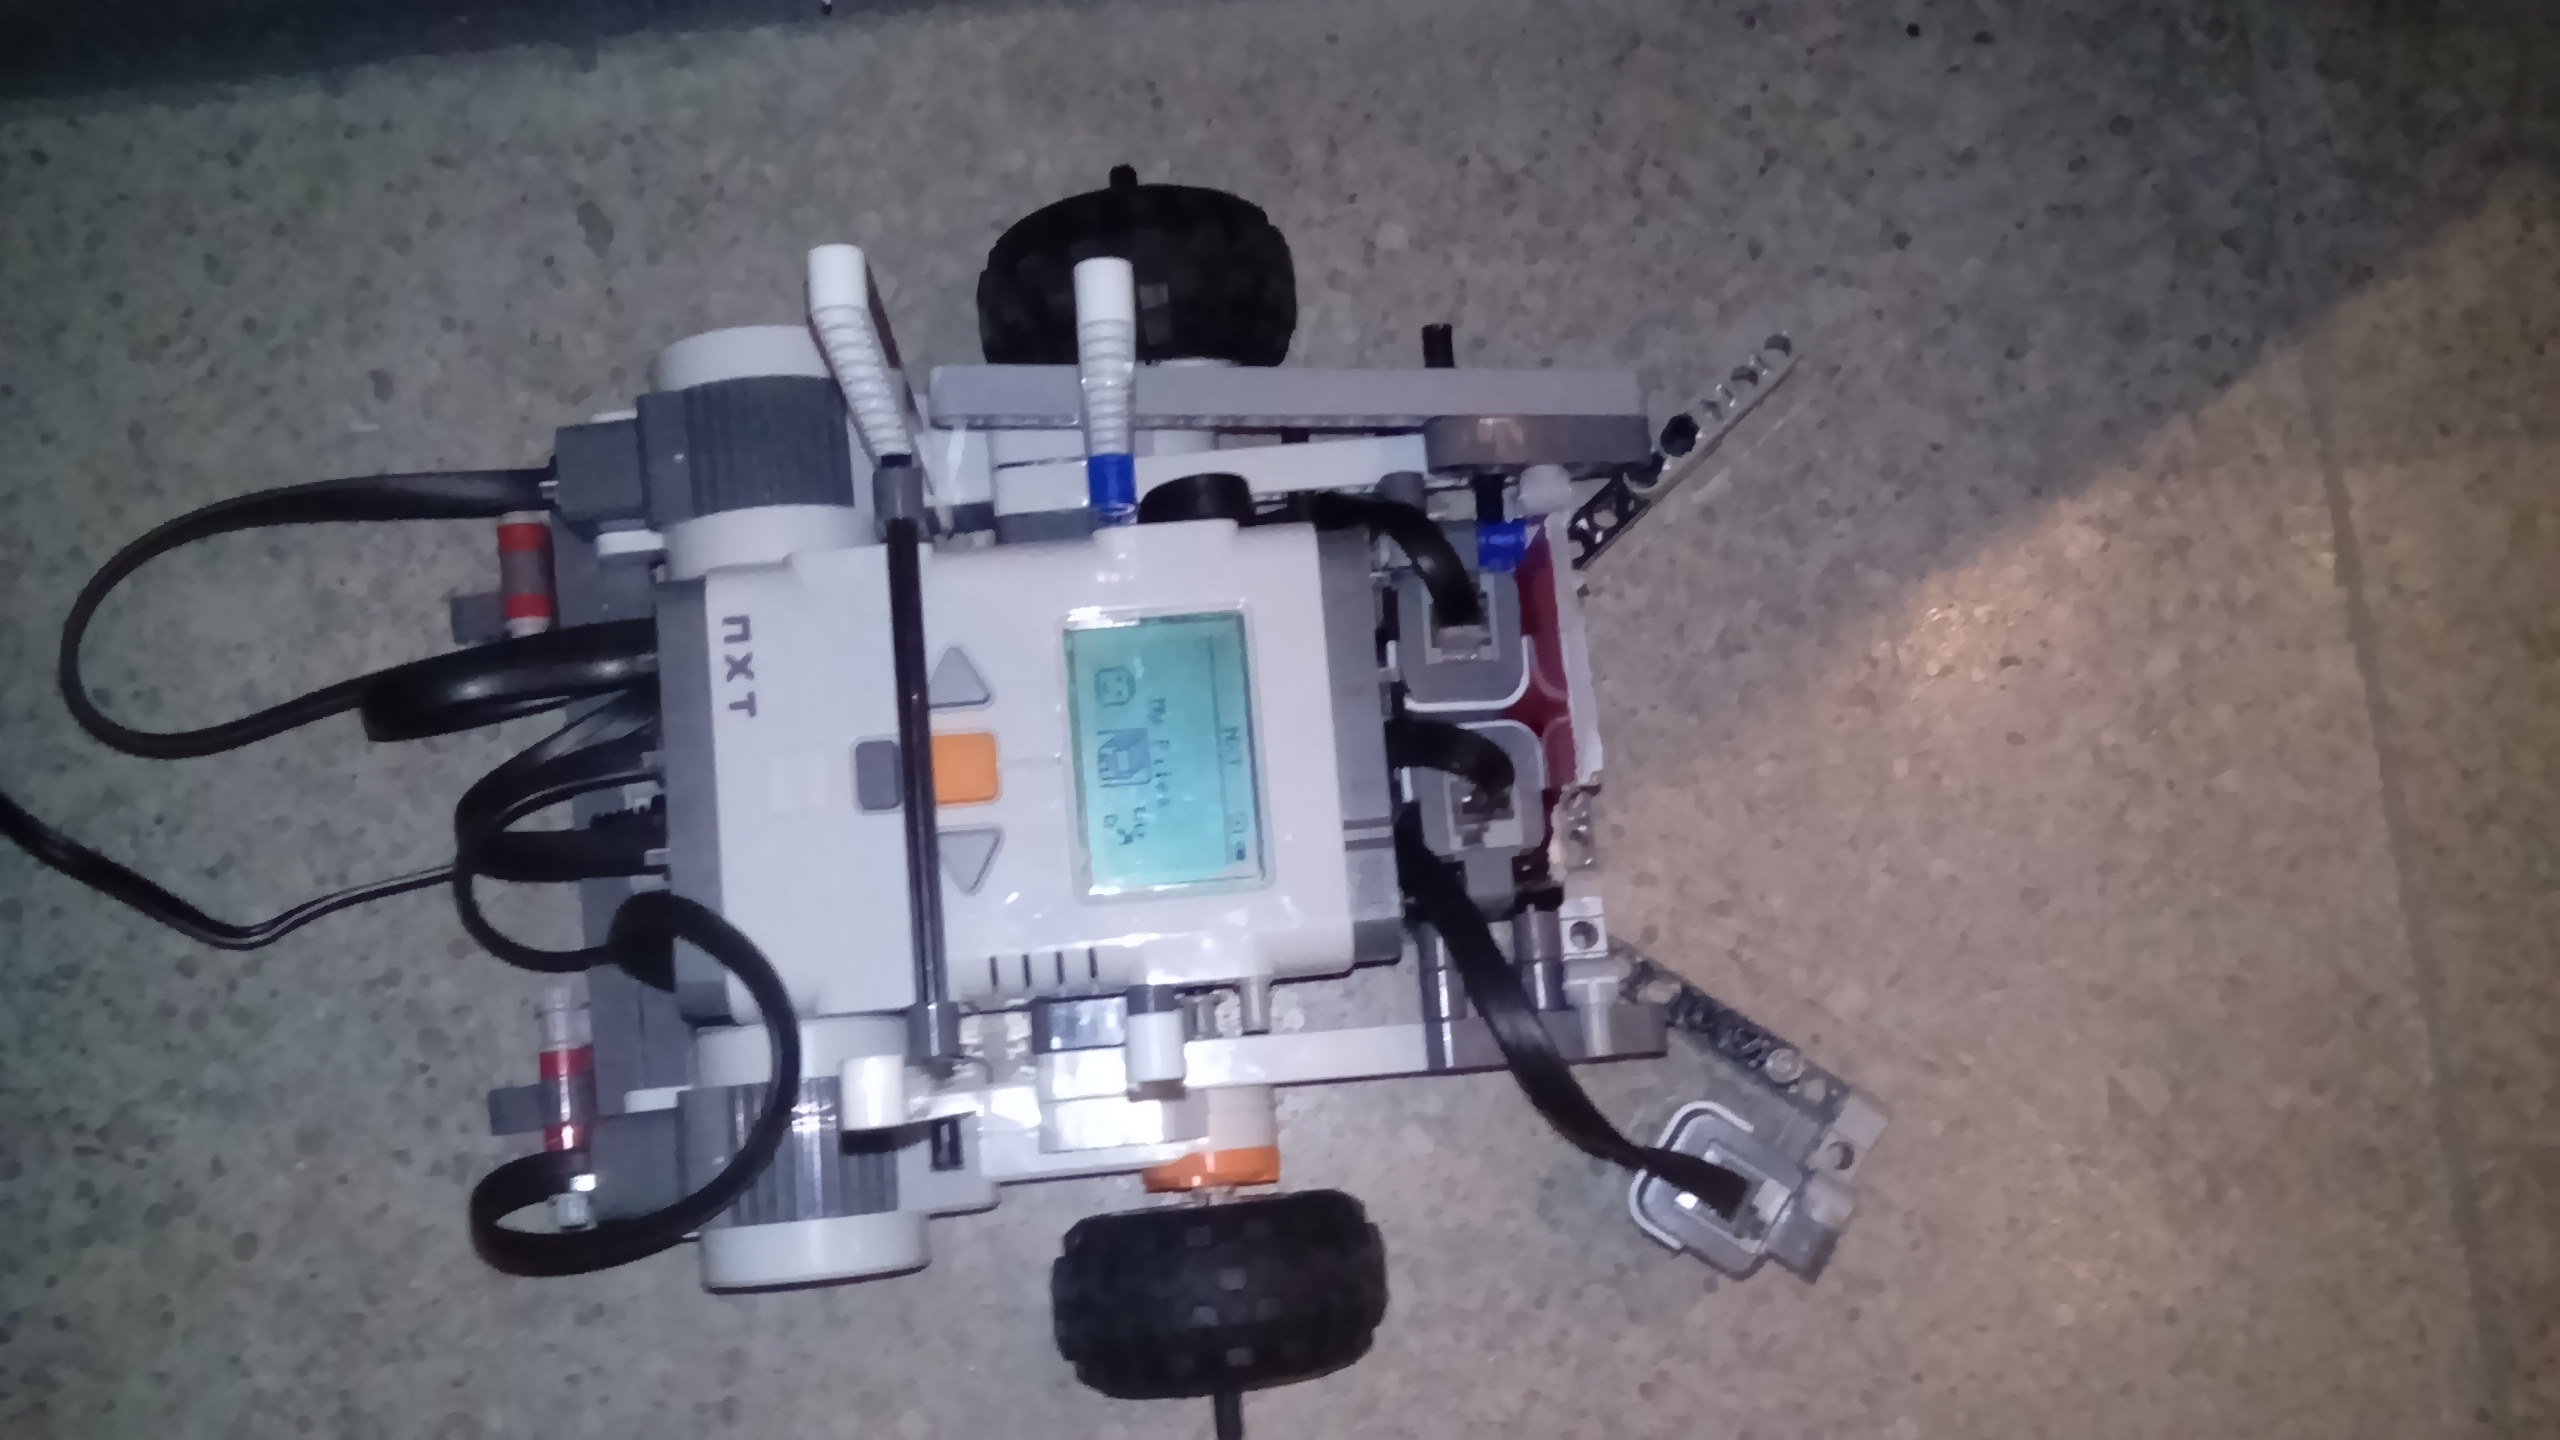
\includegraphics[scale = 0.1]{img/robot.jpg}
 \caption{Final design of the robot}
 \label{fig:final_robot}
\end{figure}


\subsection{Sensing}
In order to sense the world around it, the robot was fitted with three light sensors, the maximum number there was. Because there were only three light sensors, a decision had to be made on what to use the sensors for. All of the other types of sensors were deemed useless for this project.

It was quickly established that two sensors were needed for a line follow controller. The last sensor could then be used for a few things, e.g as indicator that a turn was completed or a detector of intersection. Both uses were tried and pros and cons were noted, and a decision was made on what was the best configuration. 

\subsection{Line Following}
To follow a line a proportional controller is used.
The light sensors gives a value to the controller and the speed of the motors are modified to be proportional to the error term between the two sensors.
This is added to a desired speed which the robot will move with, given the error is zero.

\begin{figure}
 \missingfigure{Should we add a figure which shows the robot correcting for the error?}
\end{figure}


\subsection{Turning}
To turn the robot a set of sub goals must be met.
If both motors turn in opposite direction, the robot will turn around the axis between the wheel.
This means the robot must be positioned with the axis over the intersection.
Then the robot can turn until the sensors in the middle of the robot sees the line.
As an extra calibration, the robot will then complete the turn by turning until the line is not visible anymore.
In figure \ref{fig:left_turn} is a left turn shown.
The final state of the turn is not perfect as the positioning of the sensors position cannot be placed in a perfect desired location.
This is compensated by the line following that is guaranteed to follow a turn.

\begin{figure}
 \begin{subfigure}{0.24\textwidth}
    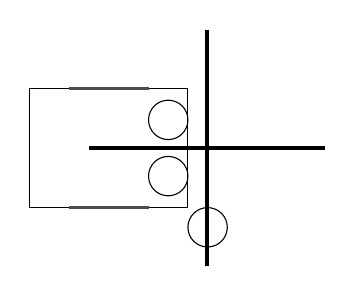
\begin{tikzpicture}
      \draw[ultra thick] (0,-1.5) to (0,1.5);
      \draw[ultra thick] (-1.5,0) to (1.5,0);
      
      \begin{scope}[rotate=-90]
	\draw node[robot,rotate=-90] at (0,-1.25) {};
      \end{scope}
    \end{tikzpicture}
  \caption{Robot at line.}\label{left_turn_a}
  \end{subfigure}
%
 \begin{subfigure}{0.24\textwidth}
    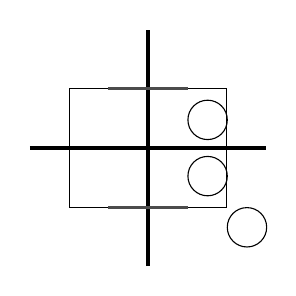
\begin{tikzpicture}
      \draw[ultra thick] (0,-1.5) to (0,1.5);
      \draw[ultra thick] (-1.5,0) to (1.5,0);
      
      \begin{scope}[rotate=-90]
	\draw node[robot,rotate=-90] at (0,0) {};
      \end{scope}
    \end{tikzpicture}
  \caption{Center at axis.}\label{left_turn_b}
 \end{subfigure}
%
 \begin{subfigure}{0.24\textwidth}
    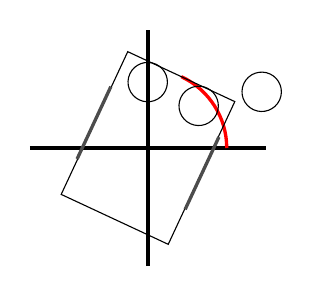
\begin{tikzpicture}
      \draw[ultra thick] (0,-1.5) to (0,1.5);
      \draw[ultra thick] (-1.5,0) to (1.5,0);
      
      \draw[red, very thick] (1,0) arc(0:65:1cm);
      \begin{scope}[rotate=-25]
	\draw node[robot,rotate=-25] at (0,0) {};
      \end{scope}
    \end{tikzpicture}
  \caption{Turn until line is found.}\label{left_turn_c}
 \end{subfigure}
%
 \begin{subfigure}{0.24\textwidth}
    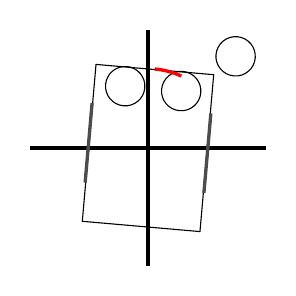
\begin{tikzpicture}
      \draw[ultra thick] (0,-1.5) to (0,1.5);
      \draw[ultra thick] (-1.5,0) to (1.5,0);
      
      \begin{scope}[rotate=-5]
	\draw node[robot,rotate=-5,name=wallE] at (0,0) {};
      \end{scope}
      
      \draw[red, very thick] (wallE.north) arc(85:65:1cm);
    \end{tikzpicture}
  \caption{Turn until line is lost.}\label{left_turn_d}
 \end{subfigure}
 \caption{A left turn for the robot.}
 \label{fig:left_turn}
\end{figure}


\section{Sokoban Solver}
Sokoban can be solved in a few different ways. 
This implementation uses an informed breadth first search algorithm in order to find the state of the puzzle, where all of the diamonds are on a goal.
In order to limit the scope of the search, dead locks and optimization of the model has been implemented.

Breadth first search algorithms take all neighboring moves and searches them before searching their children.
Informed breadth first search uses a value, like the cost of moving from one place to the other, and sorts the search list so cheapest moves are searched first.

\subsection{Model of World}
The world of Sokoban consist of a map and a series of moves.
Each move is a node in a graph which consist of the position of the man and the position of the diamonds.
To reduce the search space, only states where the position of the diamonds is known to the solver.
Each node also contains the path length, so the solver can find the optimal solution, and a pointer to the parent node so a path is linked together.
\matthias{The map consists of a map? Skal nok omformuleres}
The map consist of a representation of the map, with walls and static dead lock positions.
By having a representation of the map, finding the shortest path from the man to a diamond and detection of which diamonds are valid to push becomes possible.

The notation for the map uses J for jewels, M for the man, X for walls and G for goals.
The map using this notation can be seen in figure \ref{fig:map_notation}.
To visualize the maps and the solutions, the map is put into an existing application\cite{url:qml-sokoban}.
In figure \ref{fig:sokoban_map_2015_img} is the Sokoban map, which has been used in the competition and all tests, shown.

\begin{figure}[h]
 \centering
 \begin{subfigure}[b]{0.16\textwidth}
   \begin{minipage}{\linewidth}
\begin{verbatim}
XXXXXXXXXXXX
XX...XM.G..X
XX...X.GG..X
XXJJJ.X.GXXX
X..J....XXXX
X...X...XXXX
XXXXXXXXXXXX
\end{verbatim}
 \end{minipage}
 \caption{Map notation.}
 \label{fig:map_notation}
 \end{subfigure}~~~
 \begin{subfigure}[b]{0.3\textwidth}
  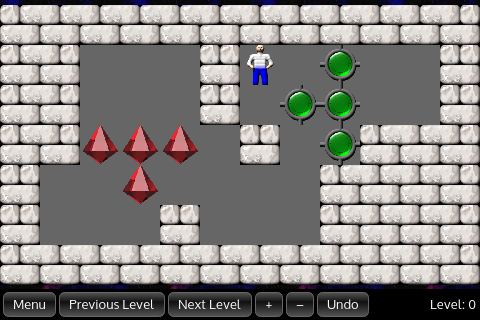
\includegraphics[width=\linewidth]{img/sokoban_2015}
 \caption{Visualized map.}
 \label{fig:sokoban_map_2015_img}
 \end{subfigure}
 \caption{Sokoban map used in competition.}
\end{figure}

A well known algorithm for breadth first search is called Dijkstra.
This algorithm was used to model to Sokoban solver.
The general algorithm can be seen in code section \ref{code:sokoban_solver}.

\begin{figure}[h]
\renewcommand\figurename{Code Section}
\centering
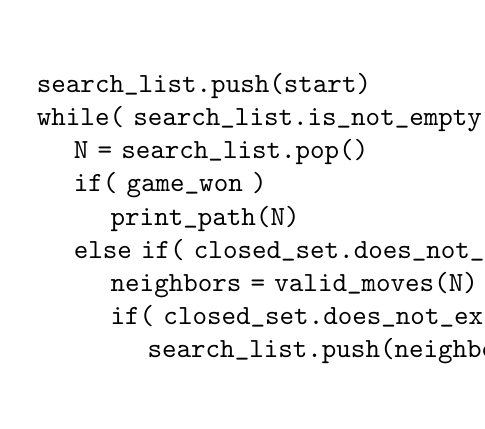
\begin{tikzpicture}
 \node[text width = 0.43\textwidth] at (0,0) {
 \begin{verbatim}
search_list.push(start)
while( search_list.is_not_empty() )
    N = search_list.pop()
    if( game_won )
        print_path(N)
    else if( closed_set.does_not_exist(N) )
        neighbors = valid_moves(N)
        if( closed_set.does_not_exist(neighbors) )
            search_list.push(neighbors)
 \end{verbatim}
 };
\end{tikzpicture}
 \caption{Sokoban solver algorithm.}
 \label{code:sokoban_solver}
\end{figure}
\matthias{Måske skal vi have med det om selve repræsentationen, med J1J2J3J4J5M og ikke det med at gemme hele mappet for at spare plads, og mappet er ligegyldigt. Det er måske logisk, men han har jo snakket om repræsentation til undervisning}
In order to easily check the if a node exist in the closed list, the closed list was implemented as a hash table.
The indexing was done as a string, using a hashing function for the diamond positions.
Each position is described as the position in a one dimension array.
% \( C = x + w \cdot y \).
The ordering of the diamonds does not matter to the solution, so the string gets sorted before the mans position is added.

%%% this can be tested by commenting out moving_rules.cpp:290; 
To test if sorting the string has any impact on the size of the graph, the solver was tested on the competition map.
Without the sorting, 467003 nodes were created before a solution was found.
With the sorting, 33160 nodes were created. 
This is a reduction of 93.37\%.

\subsection{Valid Moves}
A valid move is where a diamond has a reachable position from one direction and the other direction is either reachable or free space.
A breadth first search (wavefront) is used to this map to see all possible moves from the man's position.
Wavefront is an algorithm which takes the nearest valid moves and adds the move cost to the positions.
Consider all move directions as equal, the robot will add the cost of 1 to all neighboring fields.
In figure \ref{fig:wavefront} is the values from the wavefront shown.

\begin{figure}[h]
 \centering
 \begin{minipage}{0.1\textwidth}
\begin{verbatim}
XXXXXXXXXXXX
XX...X01234X
XX...X12345X
XXJJJ7X34XXX
X..J7654XXXX
X...X765XXXX
XXXXXXXXXXXX
\end{verbatim}
 \end{minipage}
 \caption{Wavefront on map to find valid moves.}
 \label{fig:wavefront}
\end{figure}

\subsection{Deadlock Detection}
If a diamond is pushed into a position so the map cannot be solved with any future moves the game is in a deadlock.
It is important to detect those situations to reduce the size of the graph.
There is several types of deadlocks in the game.

\begin{figure}[h]
\centering
\begin{subfigure}{0.3\textwidth}
  \centering
  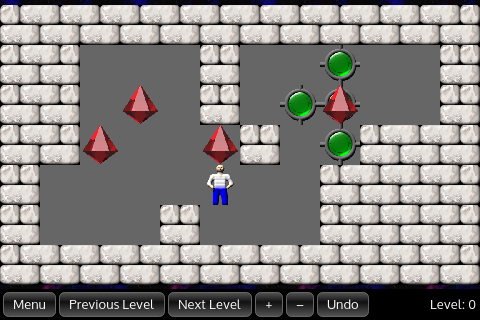
\includegraphics[width=\linewidth]{img/deadlock_corner}
  \caption{In corner.}
  \label{fig:deadlock_corner}
\end{subfigure}
%
\begin{subfigure}{0.3\textwidth}
  \centering
  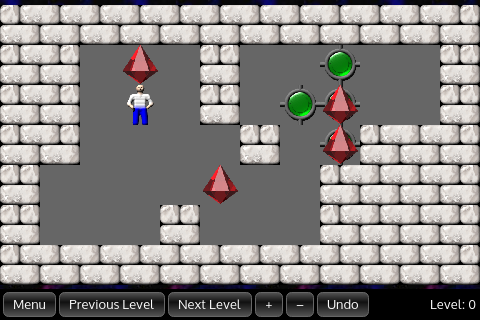
\includegraphics[width=\linewidth]{img/deadlock_wall}
  \caption{By inescapable wall.}
  \label{fig:deadlock_wall}
\end{subfigure}
\begin{subfigure}{0.3\textwidth}
  \centering
  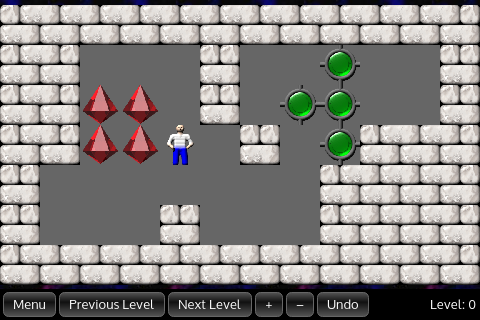
\includegraphics[width=\linewidth]{img/deadlock_diamond}
  \caption{By other diamonds.}
  \label{fig:deadlock_diamond}
\end{subfigure}
\caption{Deadlocks which the solver detects.}
\end{figure}

If a diamond is pushed into a corner, the man is unable to pull it away.
In figure \ref{fig:deadlock_corner} is a diamond locked into a corner.
Another type of deadlock is when a diamond is at a wall from which it cannot escape as seen in figure \ref{fig:deadlock_wall}.

Walls and corners can be detected when the map is loaded as they are static places it would be bad to push the diamond into.
To find those, all corners are detected.
Then a path in every direction is explored. 
If this path leads to a clearing, the diamond can be pulled away.
If the path leads to a goal, the diamond can reach a goal state.
Directions which then can directly move from one corner to another is considered an inescapable wall.
In figure \ref{fig:static_deadlocks} can the static deadlocks be seen in the map, marked with ``d''.

\begin{figure}[h]
 \centering
 \begin{minipage}{0.1\textwidth}
\begin{verbatim}
XXXXXXXXXXXX
XXdddXd...dX
XX...Xd...dX
XX...dX..XXX
Xd......XXXX
XdddXdddXXXX
XXXXXXXXXXXX
\end{verbatim}
 \end{minipage}
 \caption{Map of all static deadlocks marked with d.}
 \label{fig:static_deadlocks}
\end{figure}

Deadlocks which is created when diamonds is pushed into a cube, as seen in figure \ref{fig:deadlock_diamond} is not static places which can be avoided.
These has to be searched for at every diamond push so such situations can be avoided.

For simplicity, a diamond is not considered in a deadlock position if the diamond stands on a goal.
This leads to certain situations which cannot be detected.
Figure \ref{fig:deadlock_hard} is an example of such a situation.
Because the diamond is locked in a goal, the free space needed to push other goals in is removed and the map cannot be solved.
This situations are not detected.

Other types of deadlocks exist, but is mostly combinations of those so this is ignored.


\begin{figure}[h]
  \centering
  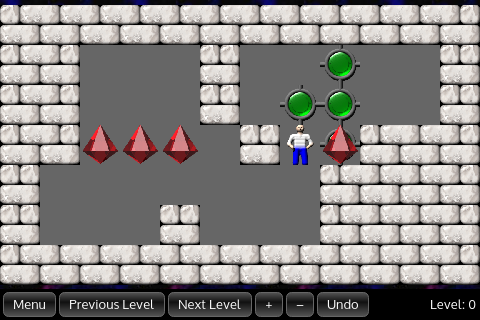
\includegraphics[width=0.3\textwidth]{img/deadlock_hard}
  \caption{Example for deadlocks which are harder to detect.}
  \label{fig:deadlock_hard}
\end{figure}

%%% To test this, comment out moving_rules.cpp:106 , dead_end = true; and deadlock would stop working
To test the strength of using deadlock detection, the sum of nodes in search list and closed list was compared.
Without any deadlock detection, the graph contained 217288 nodes.
With deadlock detection, the graph contained 33160 nodes when the solution was found.
This is a reduction of 86.76\%. 

\subsection{Robot Movement}
In order to find the optimal solution, the nodes are sorted by the path length.
This path length can be measured in the number of moves the man in the game has to make.
This will produce the shortest path between two points and the cost of moving between two places can be found by reading a single value from the wavefront map, used to detect if a diamond is movable.
This approach ignores that the robot takes time to turn and move away from a diamond.
To find the path optimal for the robot, the timing of each move is measured.
The test can be seen in the appendix.
\matthias{Tilføj test til appendix}
A variation of the wavefront algorithm is then used to find the way around the map.
At each cell, the orientation of the robot is noted and the neighboring moves are added.
Then neighboring moves are selected, taking cheapest routes first.
Then the places of the diamonds gets a cost, representing the cost in seconds it would take to move that diamond.
As all nodes are calculated at a diamond move, the cost of moving back is added to all diamonds that are not currently being pushed.
This ensures the solver knows the cost of pushing the diamond once is higher than several consecutive pushes. 
This means the output is longer in man moves, but the robot should execute the path faster.

\subsection{Performance}
To test if the solver could handle different types of maps, a set called microban \cite{url:microban} was used.
This is a set of 155 small and simple maps with a difficulty at the level expected at the competition.
In figure \ref{fig:microban_timing} is the timing of the microban levels shown.
96\% of the microban maps is solvable, and 2.7\% of those takes more than 25 seconds for the computer to solve.
In order to show the rest of the timing, these are cut off at 25 second and the timing for the test is written on the graph.
There were 6 maps which could not be solved by the solver. These are marked with red, as the user manually aborted the program when the memory consumption became too big.
The maps that was not solved have a large map and 8-16 diamonds. 
This means a lot of moves are possible and it will take a lot of memory to solve with a breadth first approach.
In those situations, it would be better to add a heuristic like the A* algorithm or solve the maps with a iterative depth first approach like IDA*.
It was evaluated that the informative breadth first approach is good enough for the competition.
\matthias{Due to the low amount of diamonds?}

\begin{figure}[h]
 \centering
 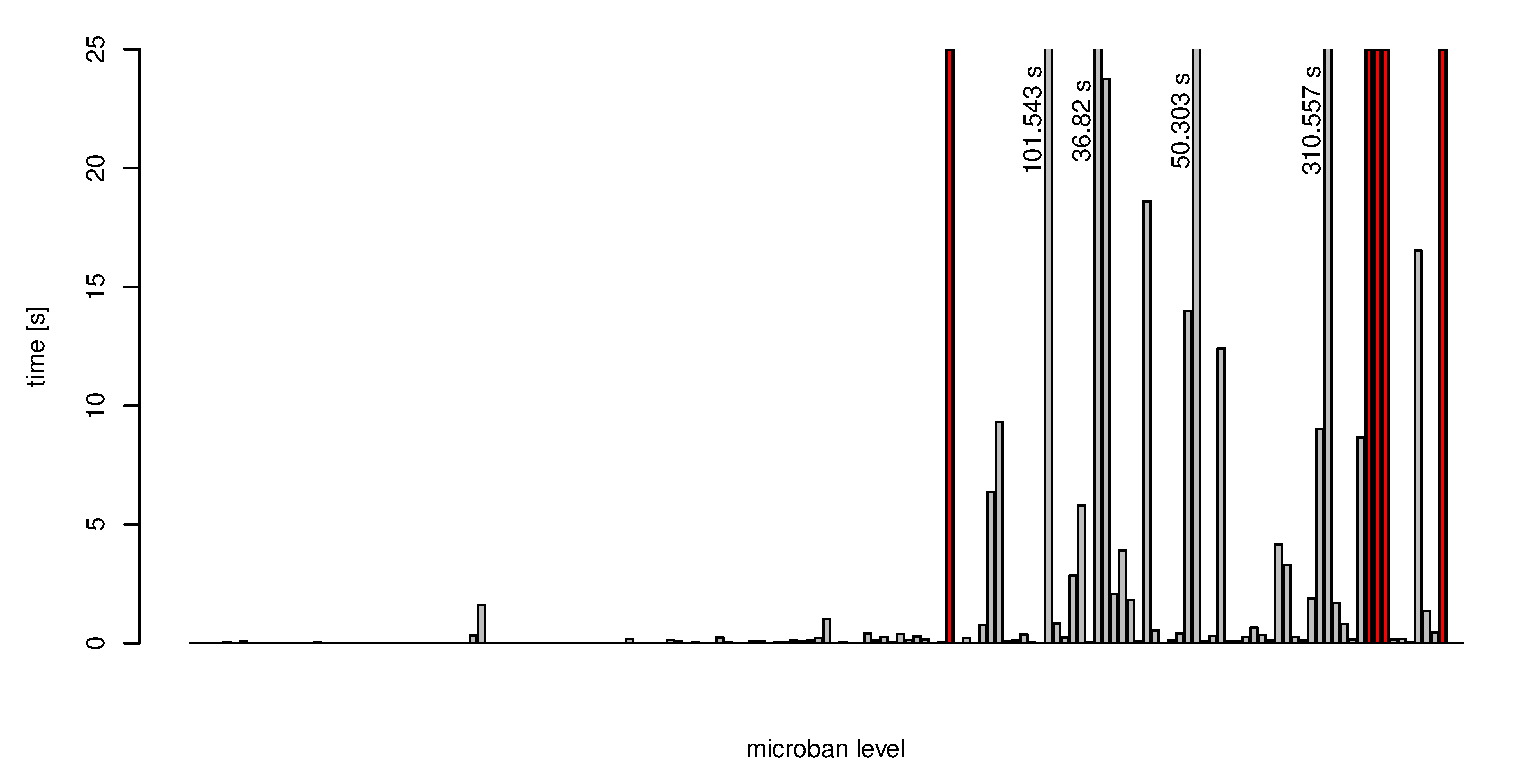
\includegraphics[width=\textwidth]{img/micoban_timing.eps}
 \caption{Timing of the microban levels. The unsolved maps are marked red.}
 \label{fig:microban_timing}
\end{figure}

%\bibliographystyle{ieeetr}
%\bibliography{src/bibtex}

\end{document}
